% ==============================================================================
% T0 Theory / FFGFT: Dokument 285 (Kapitelinhalt, DE)
% Titel: Die einheitliche kompakte Sicht (T^N, G) und die gerechnete 3-vs-6-Bruecke
% Autor: Johann Pascher
% Datum: 19. Juni 2026
% Referenzen: Dok. 206, 230, 248, 249, 270, 281, 282, 283.
% Skripte: dim_bridge_1_doubling.py, dim_bridge_2_crystallographic.py,
%          dim_bridge_3_same_ambient_fork.py
% ==============================================================================

\section*{Kurzfassung}
FFGFT und HLV reduzieren beide auf das beobachtbare $3{+}1$. Das wirft eine scharfe Frage
auf: wenn die vier Kreise von FFGFT und die sechs (plus Zeit) von HLV beide in
$\mathbb{R}^3\times\mathbb{R}_t$ enden -- sind die $3$ und die $6$ dann bloß zwei
Koordinatenbeschreibungen desselben, also nur eine mathematische Transformation? Dieses
Dokument gibt die Antwort der kompakten Sicht in \emph{einer} Notation und prüft sie
rechnerisch. Im kompakten Bild sind beide Modelle von derselben Form: ein Torus
$T^N=(S^1)^N$ mit einer endlichen Symmetriegruppe $G$ und einer Typ-I-Dekompaktifizierung
(dem Messvorgang), die einen Kreis als Zeit auswählt. FFGFT ist $(T^4,\mathbb{Z}_3)$, HLV
ist $(T^7=T^6\times S^1, A_5)$. Drei reproduzierbare Ergebnisse klären die Frage.
(1)~``$6$ ist die Verdopplung der $3$'' ist wörtlich: die ikosaedrische $6$D-Darstellung
zerfällt in $\mathbf{3}\oplus\mathbf{3'}$, die beiden $3$D-Irreps von $A_5$, die sich exakt
durch $\varphi\leftrightarrow 1-\varphi$ unterscheiden; der $6$D-Charakter ist ganzzahlig,
jeder $3$D-Block irrational ($\varphi$). (2)~Das Dreieck ist der fundamentalere, minimale
Träger: $3$-Zähligkeit ist kristallographisch und lebt in $3$D, $5$-Zähligkeit ist
nicht-kristallographisch und \emph{verlangt} die $6$D-Einbettung. (3)~Die beiden Modelle
sind \emph{durch Enthaltensein vereinbar}: die Ikosaedergruppe $A_5$ enthält die
$3$-Zähligkeit $C_3$ (beide sind Symmetrien desselben Ikosaeders), und $T^7=T^4\times T^3$,
also ist HLV das $4$D von FFGFT, erweitert um die drei Perp-Dimensionen ($7=4+3$,
$\mathrm{HLV}\supset\mathrm{FFGFT}$). Die geschützten Werte $\sqrt2$ (Koide $2/3$) und
$2/\sqrt5$ ($\varphi$) gehören zu zwei \emph{verschiedenen geschützten Geometrien} -- FFGFTs
unabhängiger $3$-Zähligkeit und HLVs $5$-Zähligkeit; die Gruppen koexistieren ($C_3<A_5$),
also keine Unverträglichkeit, und dass die cut-and-project-Familie $r(\tau)\le1$ den einen
nicht auf den anderen abbildet, zeigt nur, dass die Ineinander-Überführung die falsche
Frage ist. (Nach Dok.~283 ist $\sqrt2$ \emph{nicht} aus HLVs ikosaedrisch geschützten
Richtungen geerbt, die nur $2/\sqrt5$ geben; es ist eine eigene $3$-zählige geschützte
Wahl.) Der echte
Unterschied ist, \emph{welcher Symmetrie-Sektor physikalisch realisiert ist}: FFGFT
realisiert den minimalen kristallographischen $3$-Zähligkeits-Kern (Koide $\theta=2/9$,
empirisch bestätigt), HLV fügt die $5$-Zähligkeits-/Perp-Struktur als testbare Erweiterung
hinzu. Daher ist ``nur eine mathematische Transformation'' zu schwach (der realisierte
Sektor ist ein echtes, empirisch entscheidbares Merkmal) und ``inäquivalente Strukturen''
zu stark (sie sind vereinbar, $\mathrm{HLV}\supset\mathrm{FFGFT}$): die präzise Aussage ist
ein gemeinsamer $3{+}1$-Kern, mit HLV als ikosaedrischer Erweiterung von FFGFTs minimalem
$3$-Zähligkeits-Kern.

% ==============================================================================
\section{Anlass: beide reduzieren auf $3{+}1$ -- ist der Rest eine Transformation?}
% ==============================================================================
Dok.~270 trennt die Reduktionen von FFGFT ($T^4\to 3{+}1$) und Dok.~283 die
FFGFT$\leftrightarrow$HLV-Beziehung (eine $\mathbb{Z}_3$-Zirkulant-Brücke entlang einer
$C_3$-Achse, an der Symmetrie-Ordnung gegabelt, $\sqrt2$ vs.\ $2/\sqrt5$). HLV baut den
Raum als $6$D$\to3$D-Cut-and-Project und trägt die Zeit separat (Spiral-Time). Beide
Modelle enden somit in demselben beobachtbaren $\mathbb{R}^3\times\mathbb{R}_t$. Die
natürliche Frage ist, ob der Unterschied zwischen FFGFTs $3$ und HLVs $6$ dann bloß eine
Koordinatenwahl ist -- eine verlustfreie mathematische Transformation ein und desselben
$3{+}1$. Die Antwort braucht eine gemeinsame Notation und eine Rechnung; beides folgt. Alle
numerischen Aussagen sind mit drei kurzen Skripten reproduzierbar (\S\ref{sec:repro}).

% ==============================================================================
\section{Die einheitliche kompakte Notation $(T^N, G)$}
% ==============================================================================
In der kompakten Darstellung gibt es kein ``Raum'' gegen ``Zeit'' und kein ``intern''
gegen ``extern'': ein Kreis ist ein Kreis. Beide Modelle sind dann von einer Form:
\begin{equation}
\mathcal{M}=T^N=(S^1)^N,\qquad G\subset O(N)\ \text{wirkt,}
\end{equation}
mit einer Typ-I-Dekompaktifizierung (dem Messvorgang), die einen Kreis als Zeit wählt. Die
übrigen Kreise bleiben kompakt (diskretes Spektrum) oder projizieren (Raum, Typ~II,
Dok.~270). Die beiden Modelle sind zwei Instanzen von $(T^N,G)$:

\begin{center}\small
\renewcommand{\arraystretch}{1.3}
\begin{tabular}{@{}p{3.5cm} p{4.4cm} p{4.7cm}@{}}
\toprule
 & \textbf{FFGFT} & \textbf{HLV} \\
\midrule
kompakte Form & $T^4=(S^1)^4$ & $T^7=T^6\times S^1$ \\
Symmetriegruppe $G$ & $\mathbb{Z}_3$ (3-zählig, kristallographisch) & $A_5$ ikosaedrisch (5-zählig, nicht-kristallographisch) \\
Raum (kompakt) & $3$ Kreise & $6$ Kreise $=\mathbf{3}\oplus\mathbf{3'}$ \\
Zeit & ein Kreis (Masse-Kreis, $\tilde{T}\cdot m=1$); über die Dualität skalenverknüpft, \emph{kein} abgespaltener Faktor & ein Kreis (Spiral-Time); ein $A_5$-Singlet, der Torus \emph{faktorisiert} $T^6\times S^1$ \\
wie $G$ auf die Zeit wirkt & über $\tilde{T}\cdot m=1$ eingebunden & trivial (Singlet) \\
geschützter Invariant & $r=\sqrt2$, Koide $Q=2/3$, $\theta=2/9$ & $r=2/\sqrt5$, $\varphi$ \\
warum dieses $N_\text{Raum}$ & $3$ genügt (3-zählig kristallographisch) & $6$ nötig (5-zählig nicht-kristallographisch) \\
\bottomrule
\end{tabular}
\end{center}

Der ganze Vergleich reduziert sich auf eine Frage -- \emph{wie wirkt $G$ auf die Kreise des
Torus?} Die Etiketten ``intern/extern'' sind Dekompaktifizierungs-Sprache und haben im
kompakten Bild keinen Platz; die korrekte kompakt-konsistente Unterscheidung für den
Zeit-Kreis ist gruppentheoretisch: in HLV ist er ein $A_5$-Singlet (der Torus faktorisiert
$T^6\times S^1$, Zeit von der räumlichen Symmetrie entkoppelt); in FFGFT ist er über die
Dualität $\tilde{T}\cdot m=1$ an die anderen Kreise gebunden (kein direkter
Produktfaktor). Welcher Kreis zur beobachteten Zeit wird, ist durch den Messvorgang
festgelegt, d.\,h.\ durch die erlebte Situation des eingebetteten Beobachters (Dok.~270,
Dok.~248), nicht durch die Geometrie.

% ==============================================================================
\section{``$6$ ist die Verdopplung der $3$'' -- wörtlich (\texttt{dim\_bridge\_1})}
% ==============================================================================
Die ikosaedrische $6$D-Darstellung des Cut-and-Project zerfällt als
\begin{equation}
\mathbf{6} \;=\; \mathbf{3}\oplus\mathbf{3'},
\end{equation}
die beiden inäquivalenten $3$D-Irreps von $A_5$ (physikalisch $\oplus$ perp). Auf der
$5$-fach-Konjugationsklasse sind die Charaktere
\begin{equation}
\chi_{\mathbf 3}(g_5)=1+2\cos 72^\circ=\varphi,\qquad
\chi_{\mathbf 3'}(g_5)=1+2\cos144^\circ=1-\varphi=-\tfrac1\varphi,\qquad
\chi_{\mathbf 6}(g_5)=1.
\end{equation}
Die Verdopplung ist also wörtlich -- $\mathbf 6$ sind zwei Kopien eines $3$D-Raums -- und
der Goldene Schnitt sitzt \emph{im Split selbst}: die beiden $3$D-Blöcke unterscheiden sich
exakt durch $\varphi\leftrightarrow 1-\varphi$. Der $6$D-Charakter ist die ganze Zahl $1$,
jeder $3$D-Block irrational ($\varphi$); das ist die erste Hälfte des Grundes, warum ein
$6$D-Gitter existiert, wo ein $3$D-Gitter nicht kann (nächster Abschnitt). Dieses $\varphi$
in der Verdopplung ist HLVs $5$-Zähligkeit / $2/\sqrt5$ an der Wurzel (vgl.\ Dok.~281,
Dok.~283).

% ==============================================================================
\section{Das Dreieck ist fundamental, das Fünfeck braucht die Sechs (\texttt{dim\_bridge\_2})}
% ==============================================================================
Eine Rotation der Ordnung $n$ ist genau dann eine Gitter-Symmetrie in $2$D/$3$D, wenn
$2\cos(2\pi/n)\in\mathbb{Z}$ (kristallographische Restriktion). Ganzzahlige Werte treten
nur für $n\in\{1,2,3,4,6\}$ auf:
\begin{equation}
2\cos\tfrac{2\pi}{3}=-1\in\mathbb{Z}\quad(\text{3-zählig, kristallographisch}),\qquad
2\cos\tfrac{2\pi}{5}=\tfrac1\varphi\notin\mathbb{Z}\quad(\text{5-zählig, verboten}).
\end{equation}
Also lebt $3$-Zähligkeit ($\mathbb{Z}_3$, Koide) nativ in $3$D -- drei Dimensionen
\emph{genügen}, und das Dreieck ist der minimale, fundamentalere Träger. $5$-Zähligkeit
kann in keinem $3$D-Gitter sitzen; sie existiert nur als Projektion aus $6$D, wo sie (nach
dem vorigen Abschnitt) einen ganzzahligen Charakter erhält. Die Verdopplung $3\to6$ ist
daher keine optionale Verzierung: sie ist genau das, was die Beherbergung einer
nicht-kristallographischen Symmetrie kostet.

% ==============================================================================
\section{Dasselbe ambiente $3{+}1$: was die cut-and-project-Familie zeigt und was nicht (\texttt{dim\_bridge\_3})}
% ==============================================================================
Das cut-and-project-Verhältnis
\begin{equation}
r(\tau)=\frac{2\tau}{1+\tau^2}\le 1,\qquad r(1)=1,
\end{equation}
ist die Familie der cut-and-project-``mathematischen Transformationen''. HLVs geschützter
Invariant $2/\sqrt5\approx0{,}894$ wird bei $\tau=\varphi$ (und $\tau=1/\varphi$) erreicht.
FFGFTs $\sqrt2\approx1{,}414$ liegt \emph{über dem Maximum der ganzen Familie} und wird von
keinem $\tau$ erreicht.

\begin{figure}[h]\centering
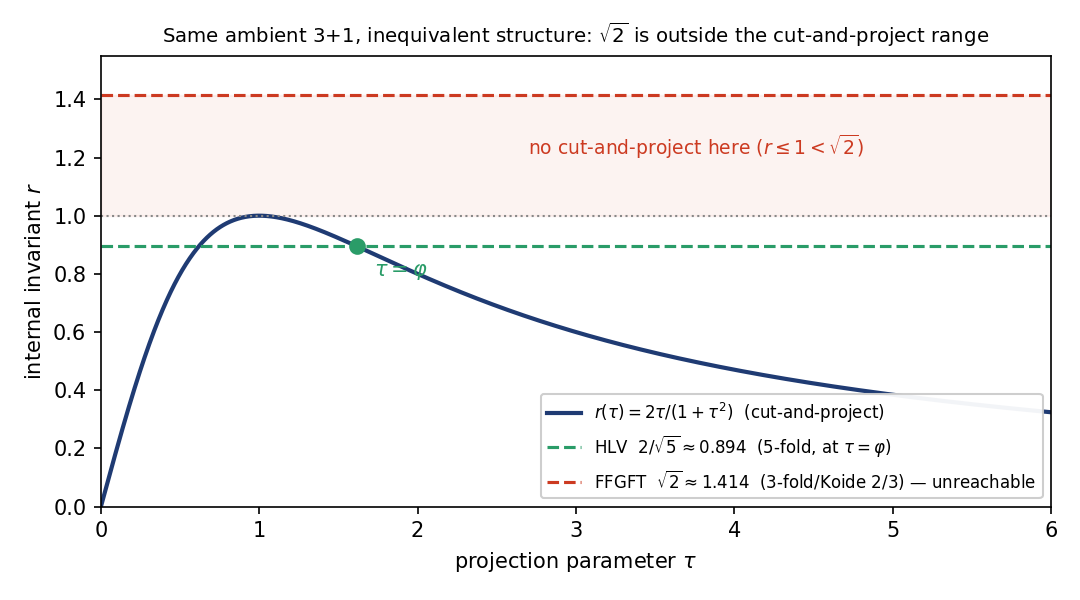
\includegraphics[width=0.92\linewidth]{../fig/fig_rtau_fork.png}
\caption{Der cut-and-project-Invariant $r(\tau)\le 1$ erreicht HLVs $2/\sqrt5$ bei
$\tau=\varphi$, aber nie FFGFTs $\sqrt2$. Dass $\sqrt2$ über dem Maximum dieser Familie
liegt, heißt nur, dass diese eine Projektion die beiden Invarianten nicht ineinander
überführt -- nicht, dass die Strukturen unverträglich sind (siehe nächster Abschnitt).}
\end{figure}

\noindent Was das zeigt -- und was nicht:
\begin{itemize}
\item \textbf{Ambientes $3{+}1$:} beide Modelle enden in $\mathbb{R}^3\times\mathbb{R}_t$;
auf der Ebene der bloßen Koordinaten-Mannigfaltigkeit ist das eine verlustfreie
Darstellungs-Transformation (Typ~III, Dok.~270/230).
\item \textbf{Die cut-and-project-Abbildung:} $\sqrt2$ liegt außerhalb des Bereichs
$r\le1$, also überführt \emph{diese} Ein-Parameter-Familie HLVs $2/\sqrt5$ nicht in FFGFTs
$\sqrt2$. Das ist eine Aussage über \emph{eine} Abbildung, \emph{kein} Beweis von
Unverträglichkeit: Vereinbarkeit heißt nicht ``überführe die beiden Invarianten ineinander'',
sondern ``bette beide in eine gemeinsame Struktur ein'' -- Thema des nächsten Abschnitts.
(Und $\sqrt2>1$ gegen $r\le1$ sind nicht streng kommensurabel, ihre Ungleichheit hier ist
bestenfalls schwaches Indiz.)
\end{itemize}

% ==============================================================================
\section{Die Vereinbarkeit: HLV enth\"alt FFGFT (\texttt{recompute\_reconcile})}
% ==============================================================================
Die entscheidende Tatsache ist gruppentheoretisch. Die Ikosaedergruppe $A_5$ \emph{enthält}
die $3$-Zähligkeit $C_3$: eine $120^\circ$-Drehung um eine $(1,1,1)$-Achse und eine
$72^\circ$-Drehung um eine Vertex-Achse sind \emph{beide} Symmetrien desselben regulären
Ikosaeders -- beide permutieren seine zwölf Ecken (\texttt{recompute\_reconcile.py}). Also
$C_3<A_5$, und auf der Dimensionsebene $T^7=T^4\times T^3$, d.\,h.
\begin{equation}
7 \;=\; \underbrace{3_{\text{phys}}+1_{\text{Zeit}}}_{\text{FFGFT }T^4}\;+\;\underbrace{3_{\text{perp}}}_{\text{HLV-Erweiterung}}.
\end{equation}
Konkret $T^4\hookrightarrow T^7$, $(x,t)\mapsto(x,0,t)$ mit $0\in T^3_{\text{perp}}$ -- eine total geod\"atische Untermannigfaltigkeit: jede FFGFT-Konfiguration ist die spezielle HLV-Konfiguration mit verschwindender Perp-Koordinate. Die Relation zwischen den Modellen ist daher \emph{Enthaltensein}, $\mathrm{HLV}\supset
\mathrm{FFGFT}$: FFGFT ist der minimale kristallographische $3$-Zähligkeits-Kern, HLV die
ikosaedrische Erweiterung, die die drei Perp-Kreise und die volle $5$-Zähligkeit hinzufügt.
Die geschützten Werte $\sqrt2$ und $2/\sqrt5$ sind Invarianten der koexistierenden $C_3$-
und $A_5$-Sektoren \emph{derselben} enthaltenden Struktur; sie müssen sich nicht, und tun
es nicht, ineinander transformieren -- und das ist kein Widerspruch. Das Enthaltensein gilt
auf der Ebene der Gruppen und Dimensionen; der \emph{geschützte} Invariant bleibt eine
eigene, realisierte Wahl -- FFGFT schützt eine unabhängige $3$-zählige Geometrie ($\sqrt2$),
HLV die $5$-zählige ($2/\sqrt5$), und (Dok.~283) HLVs geschützte Vakuum-Richtungen
enthalten $\sqrt2$ nicht. Enthaltensein macht die Modelle vereinbar, ohne sie identisch zu
machen.

\medskip\noindent\emph{Wo dies behauptet wird.} Dies alles lebt im kompaktifizierten Bild --- die Tori mit allen Kreisen kompakt, wo kein Kreis als Zeit ausgezeichnet ist. Die Br\"ucke zu physikalischen, dekompaktifizierten Observablen l\"auft \"uber den einen Schritt $S^1\to\mathbb{R}$, den Messvorgang (Dok.~270); das Enthaltensein wird also vor dem Messvorgang, im kompakten Zustand, behauptet --- nicht auf der physikalischen Zeitachse.

% ==============================================================================
\section{Auflösung}
% ==============================================================================
Die Spannung -- ``beide reduzieren auf $3{+}1$, also können die $3$ und die $6$ nur dasselbe
beschreiben'' -- löst sich nicht durch eine Gabelung, sondern durch \emph{Enthaltensein}.
Die $3$ und die $6$ teilen denselben physikalischen $3{+}1$-Kern, und die Modelle sind
mathematisch vereinbar: $\mathrm{HLV}\supset\mathrm{FFGFT}$ sowohl in der Symmetrie
($A_5\supset C_3$) als auch in den Dimensionen ($7=4+3$). Was bleibt, ist keine
mathematische Unverträglichkeit, sondern die Frage, \emph{welcher Symmetrie-Sektor
physikalisch realisiert ist}. FFGFT realisiert den minimalen, kristallographischen
$3$-Zähligkeits-Kern, und sein Invariant -- Koide $\theta=2/9$ -- ist empirisch bestätigt;
HLV fügt die $5$-Zähligkeits-/Perp-Struktur als Erweiterung hinzu, deren eigenes
Observable (das ikosaedrische / quasikristalline Kohärenz-Signal, Dok.~282/283) genau das
ist, was ein Test von HLV gegen FFGFT prüfen würde. Die frühere Formulierung wird in beide
Richtungen korrigiert: ``nur eine mathematische Transformation'' ist zu schwach (der
realisierte Sektor ist ein echtes, empirisch entscheidbares Merkmal) und ``inäquivalente,
unvereinbare Strukturen'' ist zu stark (die Einbettung $\mathrm{HLV}\supset\mathrm{FFGFT}$
existiert). Die präzise Aussage: ein gemeinsamer $3{+}1$-Kern, mit HLV als ikosaedrischer
\emph{Erweiterung} von FFGFTs minimalem $3$-Zähligkeits-Kern, der Unterschied im
realisierten Symmetrie-Sektor.

% ==============================================================================
\section{Rekursion im einheitlichen kompakten Bild: $\lambda^n$}
% ==============================================================================
Die Notation $(T^N,G)$ setzt sich in der \emph{Rekursion} fort: in beiden Modellen ist die
selbst\"ahnliche Struktur eine Dilatation um einen einzigen Eigenwert $\lambda$, die
Rekursion ist $\lambda^n$. Der Rekursions-Eigenwert ist \emph{verschieden} vom gesch\"utzten
Invarianten ($\sqrt2$, $2/\sqrt5$); beide zu verwechseln ist ein Fehler.

\textbf{FFGFT: $\lambda=\xi=4/30000$ (Dok.~270).} Die Rekursion $\xi^n$ ist einseitig
kontrahierend ($\xi,\xi^2,\dots$ verschwinden sofort) und gibt die fraktale Korrektur
\begin{equation}
D_f = 3-\xi = 2{,}999867,
\end{equation}
eine Dimension knapp unter $3$ -- fast-kristallin. Der gesch\"utzte Invariant $\sqrt2$ (Koide
$2/3$) ist eine \emph{separate} Gr\"o\ss e, nicht die Rekursions-Skala.

\textbf{HLV: $\lambda=\varphi$ (goldene Inflation).} Der ikosaedrische Quasikristall ist
selbst\"ahnlich unter der goldenen Inflation, mit der Fibonacci-Rekursion
$\varphi^2=\varphi+1$. Die Fibonacci-Substitutionsmatrix (Zeilen $(1,1)$, $(1,0)$) hat die
Eigenwerte $\varphi$ (expandierend) und $-1/\varphi$ (kontrahierend) -- dasselbe
$\varphi\leftrightarrow-1/\varphi$-Paar wie der $\mathbf 3\oplus\mathbf 3'$-Split
(physikalisch/Perp). Zweiseitig, also selbst\"ahnlich auf \emph{allen} Skalen: ein echter
Quasikristall. Der gesch\"utzte Invariant $2/\sqrt5$ ist wieder separat.

\begin{center}\small
\renewcommand{\arraystretch}{1.2}
\begin{tabular}{@{}p{2.0cm} p{2.7cm} p{5.0cm} p{2.6cm}@{}}
\toprule
 & Rekursion $\lambda$ & Charakter & gesch. Invariant \\
\midrule
FFGFT & $\xi=4/30000$ & einseitig kontrahierend, $D_f=3-\xi$ & $\sqrt2$ (Koide $2/3$) \\
HLV & $\varphi$ & zweiseitig ($\varphi,\,-1/\varphi$), $\varphi^2=\varphi+1$ & $2/\sqrt5$ \\
\bottomrule
\end{tabular}
\end{center}

\noindent Der Fork erscheint also erneut, nun in der Rekursion: $\xi$ winzig (einseitig,
fast-kristallin) gegen $\varphi$ golden (zweiseitige Inflation). Die zus\"atzliche
kontrahierende Mode ($-1/\varphi$, die Perp-Richtung) ist genau HLVs Erweiterung \"uber FFGFT,
konsistent mit $\mathrm{HLV}\supset\mathrm{FFGFT}$. In jedem Modell steuert eine Zahl sowohl
die gesch\"utzte Geometrie als auch die Rekursion.

Ein Rekursions-\emph{Phasenwinkel} (ein Analogon zu FFGFTs Koide-Winkel $\theta=2/9$) wird
hier \emph{nicht} festgelegt. Er m\"usste aus der $A_5$-Darstellung \emph{hergeleitet} werden;
das naive $2/9+1/5=19/45$ ist Numerologie, hat keine Herleitung und wird nicht \"ubernommen.
Gerechnet: \texttt{recursion\_unify.py}.

\medskip\noindent\textbf{Status von $\varphi$.} Der goldene Schnitt erh\"alt hier eine Bedeutung, die er in reinem FFGFT nicht hatte -- aber \emph{nicht} als FFGFT-Konstante, sondern als hergeleiteter Eigenwert von HLVs $5$-fach-/Perp-Sektor und damit als Marker der Grenze HLV$\setminus$FFGFT. Das ist mit Dok.~190 (P35) vertr\"aglich: dort war $\varphi^N$ das Warnbeispiel einer beliebigen Fitting-Basis ohne Vorw\"arts-Gehalt; hier ist $\varphi$ ein Eigenwert einer benannten Symmetrie (golden inflation $\varphi^2=\varphi+1$), keine in einen Exponenten gesteckte Messskala. $\varphi$ wird damit keine FFGFT-Vorhersage.

% ==============================================================================
\section{Der HLV-Phasenwinkel aus $A_5$: $\theta=0$, die Amplitude tr\"agt den Unterschied}
% ==============================================================================
Die gesch\"utzte Geometrie l\"asst sich zu einem \emph{Phasenwinkel} versch\"arfen. FFGFTs
Koide-Winkel $\theta=2/9$ ist ein Phasen-Offset im $3$-komponentigen Zirkulant
\begin{equation}
\sqrt{m_k} = 1 + A\cos\!\left(\tfrac{2\pi k}{3}+\theta\right),\qquad k=0,1,2,
\end{equation}
dessen Koide-Gr\"o\ss e $Q=(2+A^2)/6$ ist, \emph{unabh\"angig von} $\theta$. Der Modellinhalt
zerf\"allt damit sauber in Amplitude $A$ und Phase $\theta$.

\textbf{FFGFT.} $A=\sqrt2$ (die $3$-z\"ahlige gesch\"utzte Amplitude) und $\theta=2/9$ --
ein \emph{freier}, empirischer Offset ($Q=2/3$ f\"ur jedes $\theta$; $2/9$ ist der gemessene
Koide-Wert), also $Q=2/3$.

\textbf{HLV.} $A=2/\sqrt5$ (die $5$-z\"ahlige/ikosaedrische Amplitude: die $5$-fach-Eigenwert-Phasen
$\mathrm e^{\pm2\pi i/5}$ setzen sie \"uber das Skalarprodukt $1/\sqrt5$). Die gesch\"utzten
Vakuum-Richtungen sind symmetrie-starr, also gibt es \emph{keinen freien Offset}:
$\theta_{\mathrm{HLV}}=0$, was $Q=(2+\tfrac45)/6=7/15$ ergibt -- genau der Wert in der
Fork-Tabelle von Dok.~283.

$A_5$'s Eigenwert-Phasen spielen also explizite, verschiedene Rollen: die $3$-fach-Phasen
$\pm2\pi/3$ setzen das Zirkulant-\emph{Gitter} (beide Modelle); die $5$-fach-Phasen
$\pm2\pi/5$ (und $\pm4\pi/5$ in $\mathbf 3'$) setzen HLVs \emph{Amplitude} $2/\sqrt5$ --
keine freie Phase. Der ehrlich abgeleitete HLV-Phasenwinkel ist daher
$\theta_{\mathrm{HLV}}=0$, und der ganze Modellunterschied steckt in der Amplitude
(gesch\"utzter Invariant $\sqrt2$ vs $2/\sqrt5$, d.\,h.\ Koide $2/3$ vs $7/15$).

\begin{center}\small
\renewcommand{\arraystretch}{1.2}
\begin{tabular}{@{}p{1.8cm} p{1.7cm} p{3.4cm} p{2.4cm} p{1.6cm}@{}}
\toprule
 & Amplitude $A$ & Phase $\theta$ & Koide $(2{+}A^2)/6$ & Quelle \\
\midrule
FFGFT & $\sqrt2$ & $2/9$ (frei, empirisch) & $2/3$ & $3$-fach \\
HLV & $2/\sqrt5$ & $0$ (starr, gesch\"utzt) & $7/15$ & $5$-fach \\
\bottomrule
\end{tabular}
\end{center}

\noindent Das erledigt auch die naive Vermutung $\theta=2/9+1/5=19/45\approx0{,}422$: sie
trifft \emph{weder} die abgeleitete Phase ($0$) \emph{noch} das Koide-Verh\"altnis
($7/15\approx0{,}467$) und wird nirgends \"ubernommen. Das Ergebnis ist unter der
$3$-komponentigen Koide-Parametrisierung abgeleitet; $\theta_{\mathrm{HLV}}=0$ folgt aus der
Starrheit der ikosaedrisch gesch\"utzten Richtungen (vgl.\ Dok.~283). Gerechnet:
\texttt{phase\_from\_a5.py}.

% ==============================================================================
\section{Wie FFGFT ausrollt: die Dekompaktifizierung als Br\"ucke zur Beobachtung}
% ==============================================================================
FFGFT rollt aus, indem \textbf{ein Kreis des Torus $T^4$ durch den Messvorgang zur Zeit wird}
(Typ-I-Dekompaktifizierung). Die drei \"ubrigen Kreise liefern den beobachteten Raum, bleiben aber
strukturell unangetastet. Die Rekursion $\xi^n$ wird dabei zum kontinuierlichen Dilatationsfluss mit
Log-Periode $|\ln\xi|=\ln 7500\approx 8{,}92$. Entscheidend: das Ausrollen ist \emph{nicht} Teil der
Theorie, sondern die Br\"ucke zur Beobachtung (Dok.~248, Dok.~270) --- der Torus bleibt das Original,
der ausgerollte Raum ist das Bild.

\subsection{Die kompakte Form}
Im kompakten Bild ist FFGFT der Vier-Torus $\mathcal{M}=T^4=(S^1)^4$ mit $G=\mathbb{Z}_3$. Alle vier
Kreise sind \emph{gleichberechtigt} --- es gibt keine ausgezeichnete Zeit. Die drei Raum-Kreise
tragen die Eichstruktur (Connection-Laplace), der vierte ist der Masse-Kreis mit der Dualit\"at
$\tilde{T}\cdot m=1$.

\subsection{Der Messvorgang rollt einen Kreis auf (Typ I)}
Die Dekompaktifizierung ist kein mathematischer Grenz\"ubergang $S^1\to\mathbb{R}$, sondern ein
physikalischer Akt: der Messvorgang w\"ahlt einen Kreis als Zeit und rollt ihn auf. Das ist
Eigenschaft des \emph{eingebetteten Beobachters} (Dok.~248), nicht der Geometrie. Die Typ-I-Abbildung
$S^1_{\text{Masse}}\to\mathbb{R}_t$ macht aus der dualen Masse $m=1/\tilde{T}$ die Ruheenergie; dabei
wird die Windungszahl verworfen --- der informationsverwerfende Schritt, der den Beobachter in die
Zeit zwingt.

\begin{center}
\begin{tabular}{@{}p{1.5cm} p{6.2cm} p{4.3cm}@{}}
\toprule
Typ & Was passiert & Beispiel \\
\midrule
I & ein Kreis wird zur Zeit (aufgerollt, Windung verworfen) & $S^1_m\to\mathbb{R}_t$ \\
II & ein Kreis bleibt kompakt (diskretes Spektrum) & $S^1_x\to S^1_x$ (unver\"andert) \\
III & verlustfreie Koordinatentransformation & $T^4\to\mathbb{R}^3\times S^1$ \\
\bottomrule
\end{tabular}
\end{center}

Wichtig f\"ur die saubere Buchhaltung: der \emph{beobachtete} Raum $\mathbb{R}^3$ entsteht durch die
verlustfreie Koordinatentransformation (Typ III) $T^4\to\mathbb{R}^3\times S^1$ und tr\"agt
kontinuierliche Impulse; das \emph{diskrete, massentragende} Spektrum sitzt dagegen auf der kompakten
$\mathbb{Z}_3$-Faser, nicht auf der ausgerollten Achse. \enquote{Kompakt/diskret} (Faser, Massen) und
\enquote{$\mathbb{R}^3$/kontinuierlich} (Typ-III-Projektion, Raum) sind also zwei verschiedene Dinge
und nicht zu vermengen.

\subsection{Die Rekursion rollt mit aus}
Im kompakten Bild ist die Rekursion diskret, $\lambda^n$ mit $\lambda=\xi=4/30000=1/7500$. Beim
Aufrollen wird daraus ein kontinuierlicher Dilatationsfluss $t\mapsto\xi t$, $t=t_0\,\xi^s$
($s\in\mathbb{R}$) --- der Skalenfluss. Eine diskrete Skaleninvarianz im Kontinuum ist
\textbf{Log-Periodizit\"at} mit Periode $|\ln\xi|=\ln 7500\approx 8{,}92$ e-folds. Das ist eine sehr
lange Periode; daher ist FFGFT \emph{fast-kristallin}, die fraktale Korrektur winzig:
$D_f=3-\xi=2{,}9998667$. Die Ausf\"uhrung (Dilatationsfluss, Log-Periode, Verzweigung) folgt im
n\"achsten Abschnitt.

\subsection{Was \"uberlebt --- und was nicht}
\begin{center}
\begin{tabular}{@{}p{3.1cm} p{4.4cm} p{4.9cm}@{}}
\toprule
 & Kompakt ($T^4$) & Dekompaktifiziert ($\mathbb{R}^3\times\mathbb{R}_t$) \\
\midrule
Masse-Kreis & $S^1$, $m=1/\tilde{T}$ & $\mathbb{R}_t$, Ruheenergie $E=m$ \\
Raum & $3\times S^1$ & $\mathbb{R}^3$ (Typ III, kontinuierliche Impulse) \\
Massenspektrum & Eigenwerte von $S$ auf der $\mathbb{Z}_3$-Faser (diskret) & unver\"andert; $m_k=\mu_k^2\,M$, $M=1/T$ \\
Rekursion & $\xi^n$ (diskret) & $\xi^s$ (Fluss), Log-Periode $\ln 7500$ \\
Symmetrie & $\mathbb{Z}_3$ & $\mathbb{Z}_3$ (erhalten) \\
Beobachter & keiner & eingebettet (Messvorgang) \\
\bottomrule
\end{tabular}
\end{center}

Die Physik sitzt im \emph{kompakten} Bild und \"uberlebt das Ausrollen, weil sie aus \emph{Verh\"altnissen}
besteht: die $\mathbb{Z}_3$-Symmetrie (auf der Faser, nicht auf dem Torus), die Koide-Struktur
($r=\sqrt2$, $\theta=2/9$, rahmenunabh\"angig) und die Massenverh\"altnisse. Der Massenoperator
$S=\operatorname{circ}(t_0,t_1,t_2)$ \"andert sich beim Ausrollen nicht --- er lebt auf der
$C_3$-Faser, die vom Torus unabh\"angig ist; die Skala $M=1/T$ kommt aus dem Zeit-Kreis. Verworfen
wird allein die Windungszahl des aufgerollten Kreises. (Drei Zeit-Aspekte: Connection-Laplace ohne
Zeit, Prozess-Zeit \"uber den Nicht-Markov-Kern, Geometrie-Zeit \"uber $\tilde{T}\cdot m=1$; Dok.~282.)

\emph{Folge f\"ur den D7-Vergleich:} FFGFT rollt den Masse-Kreis zur Zeit und beh\"alt den
massentragenden $3$-Kern; Kr\"ugers dekompaktifizierte Variante deckt davon nur $\{3'+\text{Zeit}\}$
ab (unten). Gerechnet: \texttt{decompact\_recursion.py}.

% ==============================================================================
\section{Dekompaktifizierte rekursive Zeit: kontinuierlicher Dilatations-Fluss und Log-Periodizit\"at}
% ==============================================================================
Kompakt und dekompakt h\"angen \"uber $S^1\to\mathbb{R}$ zusammen -- den Messvorgang
(Dok.~270), und die Rekursion folgt dieser Abbildung. Im kompakten Bild ist die Rekursion die
\emph{diskrete} Dilatation $\lambda^n$ ($n\in\mathbb{Z}$): eine \emph{diskrete
Skaleninvarianz} (invariant nur unter Skalierung mit $\lambda$). Rollt der Masse-Kreis zur
nichtkompakten Zeit auf, wird aus der diskreten Rekursion ein \emph{kontinuierlicher}
Dilatations-Fluss
\begin{equation}
t\ \longmapsto\ \lambda\,t,\qquad t=t_0\,\lambda^{s},\quad s\in\mathbb{R},
\end{equation}
also der Renormierungsgruppen-/Skalenfluss. Eine diskrete Skaleninvarianz im Kontinuum ist
\emph{Log-Periodizit\"at} der Periode $|\ln\lambda|$ -- gleichwertig: komplexe
Skalenexponenten $\alpha=\alpha_0+\mathrm i\,k\,2\pi/|\ln\lambda|$.

\begin{center}\small
\renewcommand{\arraystretch}{1.2}
\begin{tabular}{@{}p{1.8cm} p{2.6cm} p{6.2cm}@{}}
\toprule
 & kompakt & dekompaktifiziert \\
\midrule
FFGFT & $\xi^n$ (diskret) & Fluss $t\to\xi t$; Log-Periode $|\ln\xi|=\ln 7500\approx8{,}92$ \\
HLV & $\varphi^n$ (diskret) & Fluss $t\to\varphi t$; Log-Periode $\ln\varphi\approx0{,}481$ \\
\bottomrule
\end{tabular}
\end{center}

\noindent Der Fork bleibt in der dekompaktifizierten Zeit erhalten. \textbf{FFGFT}: eine
Log-Periode von $\approx8{,}9$ e-folds -- sehr lang, also kaum log-periodisch; fast-kristallin.
Es ist dieselbe diskrete Skaleninvarianz, die $D_f=3-\xi$ erzeugt. \textbf{HLV}: eine
Log-Periode von $\approx0{,}48$ e-folds -- kurz und dicht; ein voller Quasikristall,
selbst\"ahnlich auf jeder Skala.

FFGFTs \emph{Rekursion $R$} ist genau dieses Objekt: diskret ($\xi^n$) im kompakten Bild, ein
kontinuierlicher RG-/Skalenfluss nach der Dekompaktifizierung -- das $R$ liest sich beidseitig
(Rekursion $\leftrightarrow$ Renormierungsfluss). Gerechnet: \texttt{decompact\_recursion.py}.

\subsection{Marcels dekompaktifizierte Variante: der overdamped Kern ist das dekompaktifizierte leere Fenster}
Die Verdopplung hat zwei Zweige; die Dekompaktifizierung $S^1\to\mathbb{R}$ (der Messvorgang)
macht aus jedem einen kontinuierlichen Skalenexponenten $\alpha=\ln\mu$:
\begin{center}\small\renewcommand{\arraystretch}{1.15}
\begin{tabular}{@{}l r l@{}}
\toprule
Zweig & $\operatorname{Re}\alpha$ & dekompaktifizierter Charakter \\
\midrule
expandierend $\varphi$ (der D4-Kern, Massen) & $+0{,}481$ & relevant; Koh\"arenz / Revival (Back-flow $5{,}125$) \\
kontrahierend $-1/\varphi$ (das $3'$-Fenster) & $-0{,}481$ & irrelevant; abklingend / overdamped \\
\bottomrule
\end{tabular}
\end{center}
\noindent Beide teilen $|\ln\varphi|\approx0{,}481$; nur das Vorzeichen unterscheidet sich. Der
abklingende Zweig ist genau HLVs overdamped, abklingender Kern (Dok.~282--284):
\textbf{Marcels overdamped Kern ist das dekompaktifizierte leere Fenster} --- das kompakte
\enquote{leere $3'$} ($\to0$ diskret) und das dekompaktifizierte \enquote{overdamped, abklingend}
($\operatorname{Re}\alpha<0$, $\to0$ kontinuierlich) sind dasselbe Objekt auf den zwei Seiten der
Messung.

Entscheidend: die Containment-Relation \"uberlebt die Dekompaktifizierung. Dekompaktifiziertes D7
ist \emph{nicht} der overdamped Kern allein: es ist der D4-Kern (der relevante, koh\"arenztragende
$\varphi$-Zweig mit den Massen und dem Revival $5{,}125$) \emph{plus} das $3'$-Fenster (der
irrelevante overdamped Zweig). Der D4-Kern bleibt in dekompaktifiziertem D7 als dessen relevanter
Sektor enthalten; Marcels Kern ist das \emph{zus\"atzliche} Fenster, nicht das Ganze. Das ist nur
das dekompaktifizierte Bild von $T^4\subset T^7$.

Zwei Vorbehalte. Die Identifikation \enquote{overdamped Kern $=$ dekompaktifiziertes Fenster} ist
eine vorgeschlagene Lesart (beide sind der abklingende, nicht-diskriminierende Sektor), kein Satz.
Und weil die Dekompaktifizierung der Messvorgang ist (informationsverwerfend), sitzt dieser Zweig
konstruktionsbedingt auf der null-reproduzierbaren Seite: der diskriminierende Inhalt (Revival
$5{,}125$) liegt im relevanten D4-Kern, nicht im overdamped Kern. Gerechnet:
\texttt{decompact\_branches.py}.

\subsection{Bezug zu Kr\"ugers HLV-Kernel und Claim-State-Note}
Kr\"ugers tats\"achlicher HLV-Memory-Kernel ist eine positive Mischung abklingender Exponentiale,
$K(t)=\sum_i w_i\,\tau_i^{-1}e^{-t/\tau_i}$ (Kr\"uger, \emph{Pre-Registered Null-Model Benchmark
for HLV-Constrained Memory Kernels}, 2026). Jeder Mode ist reines Abklingen (Skalenexponent
$\operatorname{Re}<0$), der Kernel \emph{ist} also das dekompaktifizierte kontrahierende
$-1/\varphi$-Fenster des vorigen Unterabschnitts. Entscheidend: Kr\"ugers eigener
vorregistrierter Benchmark findet diesen Kernel von einem generischen positiven
Zwei-Exponential-Kernel statistisch ununterscheidbar --- das Uniqueness-Gate bleibt falsch,
\enquote{not a unique physical signature.} Das ist die null-reproduzierbare Seite, durch sein
Ergebnis belegt, nicht blo\ss\ von uns behauptet.

Der volle HLV-Operator f\"ugt dem positiven Kernel einen skew-adjungierten Phasenkanal
($J^\top=-J$) hinzu. Der skew-adjungierte (nicht-Gradienten-)Teil ist genau die Struktur, die
seine Claim-State-Note f\"ur anhaltende Rekurrenz fordert --- reiner Gradientenfluss tr\"agt keine
Zyklen --- und ist das Analogon zum relevanten, oszillatorischen FFGFT-Revival ($5{,}125$); der
abklingende Kernel ist das overdamped Fenster. Die zwei Sektoren passen: diskriminierender Inhalt
sitzt im rekurrenten/koh\"arenten (nicht-Gradienten-)Teil, nicht in der abklingenden Magnitude.

Ein dritter, sch\"arferer Bezug kommt vom Path-Memory-Komparator (De~Jesus, HICE-MEM, f\"ur
Kr\"uger): zeitliche Ordnung ist antisymmetrisch, $\mathrm{Area}(P)=\sum_{i<j}[A_i,A_j]$ mit
$\mathrm{Area}(P^{\mathrm{rev}})=-\mathrm{Area}(P)$, also sind Magnitude und Spektrum einer
\emph{einzelnen} Historie \emph{gerade} unter Umkehr --- das anti-hermitesche Spektrum
$\{i\lambda\}\mapsto\{-i\lambda\}$ ist dieselbe Menge. Das Ordnungs-Vorzeichen geht verloren,
solange man es nicht gegen eine orientierte Referenz (eine zweite Historie) kontrahiert. Das ist
dieselbe Struktur wie die Messung $S^1\to\mathbb{R}$, die die Windung verwirft, w\"ahrend die
Magnitude \"uberlebt: der diskriminierende Inhalt ist relational, nicht einzel-historisch.

Schlie\ss lich der Claim-State. Kr\"ugers Klärungs-Note (2026) trennt kompakte interne
Spiral-Time, SI-Messzeit und den Signal-Index $\Delta\Phi_{\mathrm{sig}}$ und verbietet ihre
Gleichsetzung ohne explizite Projektions-/Kalibrierungskarte $K$ --- dieselbe Disziplin wie
\enquote{Struktur $\neq$ Physik ohne Karte.} Es wird keine Identit\"at der beiden Spiral-Begriffe
und keine Holonomie behauptet: Kr\"ugers Spiral-Time tritt als beschr\"ankter kinetischer
Vorfaktor $A_\psi(t)$ am Kernel (Benchmark) und als triadische kompakte Koordinate
$\theta\in S^1$ (Note) auf, keiner davon ist die log-periodische Log-Spirale der
dekompaktifizierten Rekursion. Gerechnet: \texttt{marcel\_kernel\_match.py}.

\subsection{Kr\"ugers ausgerollte Variante deckt nur $\{3'+\text{Zeit}\}$ ab --- nicht den vollen D7}
Eine Einordnung der dekompaktifizierten Seite, \emph{ohne} \"Ubernahme von Kr\"ugers Formeln. Das
kompakte FFGFT-Resultat --- $6=3\oplus3'$ als fraktale innere Rekursion, rein aus dem Goldenen
Schnitt (Fibonacci-Operator, Eigenwerte $\varphi$ expandierend / $-1/\varphi$ kontrahierend) ---
ist hergeleitet und skriptgedeckt (\texttt{recursion\_doubling\_empty.py},
\texttt{verify\_recursion\_doubling.py}, $11/11$) und steht unabh\"angig von HLV. Es wird hier nicht
angetastet; der folgende Vergleich ber\"uhrt es nicht.

Kr\"ugers j\"ungste dekompaktifizierte Konstruktion (\emph{Recursive Spiral-Time Nesting as a Route
to a Six-Dimensional Host Carrier}, 2026, mit den null-gegateten L\"aufen Zenodo
20770402\,/\,20772007) erreicht einen $6$D-Host \"uber eine \emph{Stabilit\"ats-Selektion} (eine
Spektrall\"ucke), \emph{nicht} \"uber $\varphi$ --- ein anderer Mechanismus, kein
$\varphi$-Ersatz. F\"ur die Vereinbarkeit z\"ahlt jedoch nicht der Mechanismus, sondern \emph{was
die ausgerollte Variante f\"ullt}: ausschlie\ss lich den \textbf{leeren} Sektor. Sein abklingender
Kern ist das dekompaktifizierte $-1/\varphi$-Fenster (oben); sein Host-Sektor ist candidate-only und
massenlos (\enquote{host dimension, not masses}); und seine kompakte Zeit erf\"ullt
$\chi(t)\neq\ln t$ (Kl\"arungs-Note), ist also nicht die Log-Spirale der FFGFT-Rekursion.

Die Volltext-Fassung (2026) erg\"anzt die downstream-Kette BD3--BD5 (Zenodo 20773678): nativer
endlicher Carrier (BD3), low-q-Lorentz/EFT-Pre-Screen (BD4) und semantischer Transfer (BD5). Sie
f\"ugt nur weitere Struktur hinzu und erreicht weiterhin keine Physik --- BD4-HARD weist das
low-q-Verhalten selbst als \emph{carrier-bedingt, nicht HLV-spezifisch} aus (matched nulls bestehen
ebenso), BD0/BD1 bleiben negativ. Das verst\"arkt das $\{3'+\text{Zeit}\}$-Bild: der Carrier ist
elaboriertere, aber massenlose Struktur. (Die Nesting-Idee selbst datiert Kr\"uger auf die
Januar-2026-HLV-Grundlage, Zenodo 18255159.)

In D7-Buchhaltung --- $7=[\,3\text{-Kern (kristallographisch, Massen)}+\text{Zeit}\,]+3'$ --- rollt
seine Variante damit nur \textbf{$3'$ + Zeit} aus: das leere Perp-Fenster plus die ausgerollte
Zeitachse ($S^1_m\to\mathbb{R}_t$, gemeinsam). Der massentragende kristallographische $3$-Kern
($\varphi/\xi$, $\sqrt2$, Koide $2/3$) wird von ihr \emph{nicht erreicht} und bleibt FFGFTs.
Genaugenommen ist sein HLV --- dekompaktifiziert realisiert --- \emph{nicht} der vollst\"andige
D7-Raum, sondern der Untersektor $\{3'+\text{Zeit}\}$; den vollen D7 (Mass-Kern $+$ Zeit $+\,3'$)
realisiert FFGFT.

Daraus die Vereinbarkeit, knapp: seine Seite $\subseteq$ FFGFTs $\{3'+\text{Zeit}\}$. Der formale
Containment $T^7\supset T^4$ ($A_5\supset C_3$) bleibt; er wird hier nur pr\"azisiert, \emph{wo}
Kr\"ugers ausgerollte Konstruktion tats\"achlich sitzt. Kompatibel ist das, \emph{solange er die
candidate-only-Linie h\"alt} (seine Gates B0--B7); \"uberz\"oge er sp\"ater
(\enquote{$6$D-Host $=$ physische Raumzeit mit Massen}), w\"are die Vereinbarkeit neu zu pr\"ufen ---
aktuell tut er das ausdr\"ucklich nicht. Abgedeckt durch \texttt{decompact\_branches.py} und den
Leere-Satz oben; f\"ur seine Formeln ist kein neues Skript n\"otig.

% ==============================================================================
\section{Was der d7-Sektor berechnet: Massen aus $\xi$, Spektren aus $\varphi$}
% ==============================================================================
In Analogie zu $\xi$ fragt man, was das d7-Modell ($T^7$, $A_5$) berechnet. Die ehrliche
Antwort lautet: \emph{keine Massen}. Massen sind der Output des kristallographischen
$3$-fach-Sektors mit $\xi$, den d7 bereits enth\"alt (HLV~$\supset$~FFGFT); d7 reproduziert sie
\emph{durch} seinen FFGFT-Unterteil, nicht als neuen Inhalt. Die \emph{zus\"atzliche}
d7-Struktur ($5$-Z\"ahligkeit, Perp-Richtungen, $\varphi$) ist genau der Teil, der keine Massen
tr\"agt. Was er stattdessen tr\"agt:

\begin{center}\small\renewcommand{\arraystretch}{1.2}
\begin{tabular}{@{}p{3.4cm} p{5.6cm} p{2.8cm}@{}}
\toprule
Gr\"o\ss e & d7 / $5$-fach-Output & Status \\
\midrule
gesch\"utzte Amplitude & $2/\sqrt5$, Koide-Analogon $Q=7/15$ & hergeleitete Zahl \\
Phase & $\theta_{\mathrm{HLV}}=0$ (kein freier Koide-Winkel) & hergeleitet \\
Rekursionsskala & $\varphi$; Turm $\varphi^n$; Log-Periode $\ln\varphi\approx0{,}481$ & hergeleitet \\
Spektrum & aperiodisches Quasikristall-L\"uckenspektrum, $\varphi$-Skalierung & Diskriminator (271/283) \\
\bottomrule
\end{tabular}
\end{center}

\subsection{Warum das Spektrum hier nicht zu Massen f\"uhrt}
FFGFTs Massen sind selbst spektral -- Eigenwerte des $T^4$-Verbindungs-Laplace, die
Koide-Zirkulant-Niveaus -- die Frage ist also berechtigt; die Antwort h\"angt davon ab,
\emph{welches} Spektrum. Eine Masse ist ein scharfes, isoliertes Niveau, also braucht das
Ablesen von Massen ein \emph{diskretes Punktspektrum}. Die $3$-Z\"ahligkeit ist
gittervertr\"aglich ($2\cos(2\pi/3)=-1\in\mathbb{Z}$): sie schlie\ss t auf einem periodischen
Torus zu genau drei scharfen Eigenwerten $\{-1,-1,2\}$ -- dem Triple. Die $5$-Z\"ahligkeit ist
gitterun\-vertr\"aglich ($2\cos(2\pi/5)=1/\varphi\notin\mathbb{Z}$): kein periodisches Gitter
tr\"agt sie, ihr einziger Tr\"ager ist ein aperiodischer Quasikristall, dessen Spektrum
\emph{singul\"ar-stetig} (Cantor-artig) ist -- eine dichte L\"uckenmenge, selbst\"ahnlich unter
$\varphi$, ohne isolierte Niveaus (eine Fibonacci-Kette zersplittert auf jeder Skala in
L\"ucken, gegen die wenigen B\"ander der periodischen Kette; \texttt{spectrum\_to\_mass.py}).
Es gibt kein ausgezeichnetes Triple zum Ablesen. Daher braucht \enquote{Spektrum~$\to$~Masse}
ein Punktspektrum, also einen periodischen / kristallographischen Tr\"ager -- und der einzige
kristallographische Teil von d7 ist sein $3$-fach-Kern, also FFGFT. Der Weg kehrt stets nach
FFGFT zur\"uck; das echt d7-eigene (aperiodische) Spektrum kann keine Massen liefern. Und ein
dichtes selbst\"ahnliches Spektrum hat ein Niveau nahe \emph{jeder} Zahl, also \enquote{passt}
$\varphi^N$ zu allem -- die P35-Numerologie-Falle (Dok.~190, R44): die Reichhaltigkeit des
Quasikristall-Spektrums ist genau das, was das Ablesen einer Masse gehaltlos macht, w\"ahrend
die Sparsamkeit des diskreten Torus-Spektrums einen Eigenwert dort zur echten Vorhersage macht.

\subsection{Informationsgehalt: Struktur-Spektrum gegen Energie-Spektrum}
Der vorige Punkt darf \emph{nicht} als \enquote{das Quasikristall-Spektrum tr\"agt keine
Information} gelesen werden. Es tr\"agt sehr wohl welche -- ein Quasikristall hat \emph{zwei}
Spektren verschiedenen Typs. Das \emph{Struktur-/Beugungsspektrum} $S(q)=|\sum_n e^{\mathrm i q
x_n}|^2$ ist \emph{rein punktf\"ormig}: scharfe Bragg-Spitzen an $\varphi$-Modul-Positionen,
hier $\approx21\times$ \"uber dem Rausch-Boden eines Zufalls-Nullmodells gleicher Zusammensetzung
(\texttt{quasicrystal\_information.py}). Diese scharfe, vom Nullmodell unterscheidbare Ordnung
\emph{ist} die Information -- genau HLVs Substrat-Unterscheidbarkeit, und die steht. Das
\emph{Energie-/Laplace-Spektrum} ist das singul\"ar-stetige (Cantor-artige) aus dem vorigen
Unterabschnitt; ihm fehlen die scharfen Niveaus, daher keine Massen. Die beiden sind
verschiedene Objekte: die Information liegt in der relationalen langreichweitigen Ordnung
(Struktur-Spektrum), nicht in einzelnen Energie-Niveaus (die Energiezust\"ande sind
kritisch / fraktal, keine sauberen Knoten). Der P35-Vorbehalt ist daher eng: gehaltlos ist
allein das Anpassen \emph{einer einzelnen Zielzahl} als $\varphi^N$; das Struktursignal nicht.

\noindent\emph{Ehrlicher Rest.} Die Stelle, an der die FFGFT-Analyse ein HLV-Signal
\emph{null-reproduzierbar} fand, ist der \emph{zeitliche} \"uberd\"ampfte Ged\"achtniskern
(Dok.~282--284, biexponentiell, nicht-identifizierbarer Sektor) -- die Zeit-Domäne, ein anderes
Objekt als das r\"aumliche Struktur-Spektrum. Also: r\"aumliche Struktur informativ (HLVs Punkt
gilt); zeitlicher \"uberd\"ampfter Kern = der stehende Kritikpunkt. Die unterscheidende
Information lebt im strukturell-spektralen Signal (rein-punktf\"ormige Beugung;
periodisch-gegen-aperiodisch) -- der Diskriminator aus Dok.~271/272/283. FFGFT und HLV sind sich
einig, \emph{wo} die Information sitzt (in der Struktur); die Kritik betraf eine andere
(zeitliche) Behauptung.

\subsection{Die eine Stelle, an der d7 Massen ber\"uhren k\"onnte (Vermutung)}
Der $6=3\oplus3'$-Split l\"asst die Perp-Darstellung $3'$ (Charakter $1-\varphi=-1/\varphi$) als
\emph{zweite} Triplett-Position; FFGFT realisiert die eine $3$ (geladene Leptonen, Koide $2/3$),
die $3'$ ist leer. \emph{Falls} dort ein physikalisches Triple s\"a\ss e, w\"are seine
Vorhersage $Q=7/15$ -- ein falsifizierbares Ziel, keine hergeleitete Teilchenmasse. Gerechnet:
\texttt{what\_d7\_computes.py}.

% ==============================================================================
\section{Das Elektron-Mode in D7: die Einbettung existiert, das Massen-Label ist C$_3$-Rahmen}
% ==============================================================================
Eine nat\"urliche Konsistenzfrage: wird ein Mode in D4 als Elektron abgelesen, so muss es ein
Bild in D7 haben, da $T^4\subset T^7$. Das hat es. Das Elektron-Mode hebt sich zum D7-Mode mit
gleicher Windung auf den vier D4-Kreisen und Null-Windung auf den drei Zusatzkreisen; da es ganz
im D4-Block sitzt, bleibt sein Laplace-Eigenwert --- die Masse --- unver\"andert. Die
\"Ubersetzung ist die Einbettung selbst.

Das widerspricht nicht \enquote{Massen brauchen den D4-Kern.} Das scharfe Label
\enquote{Elektron} ist eine C$_3$-(kristallographische) Aussage, keine $A_5$-Aussage: das
Elektron-Mode ist Eigenvektor der $3$-Z\"ahligkeit. Die volle D7-Symmetrie ist $A_5$, deren
$5$-fach-Elemente nicht mit C$_3$ kommutieren --- sie drehen das Elektron-Mode in eine
Myon/Tau-Mischung. Unter einer echten ikosaedrischen $5$-Drehung beh\"alt die Elektron-Richtung
$0{,}762$ ihres Gewichts und leckt $0{,}238$ in die $\mu/\tau$-Richtungen
(\texttt{electron\_mode\_in\_d7.py}). Im vollen $A_5$-Rahmen ist \enquote{Elektron} also kein
scharfer Eigenzustand; um es als Elektron (scharfe Masse) zu lesen, w\"ahlt man die
C$_3$-Eigenbasis --- die Einschr\"ankung auf den kristallographischen Block, also
\enquote{zur\"uck nach D4.} Die Entsprechung ist die Einbettung; die Massen-Ablesung ist die
Rahmen-Wahl; beides ist dieselbe Aussage.

Zwei Absicherungen. Das Mischen ist ein Basiswechsel, kein Verschmieren: die $5$-Z\"ahligkeit
dreht den Bezeichnungs-Rahmen und zerst\"ort das physikalische Mode nicht, das in jedem
C$_3$-Rahmen perfekt scharf bleibt. Und das Mode bleibt im periodischen \enquote{$3$}-Block
(Punktspektrum) --- es leckt nicht in den aperiodischen $3'$-Sektor; die $5$-Z\"ahligkeit dreht
nur $e\leftrightarrow\mu\leftrightarrow\tau$ innerhalb der physikalischen \enquote{$3$}.
Schlie\ss lich ist es wieder der Messvorgang (Dok.~270/248), welcher Rahmen als $3$-Z\"ahligkeit
z\"ahlt: das Mode existiert rahmenunabh\"angig in D7, das scharfe Teilchen-Label ist
rahmenabh\"angig.

% ==============================================================================
\section{Das 3$'$ ist die erste Rekursion: warum Rekursionsrichtungen im kompakten Bild leer sind}
% ==============================================================================
Die Spaltung $6=3\oplus3'$ und die goldene Rekursion sind nicht zwei Tatsachen, sondern eine:
die Verdopplung \emph{ist} die einmal angewandte Rekursion. Dieser Abschnitt macht das explizit
und zieht die Folge f\"ur das leere $3'$.

\subsection{Die Verdopplung ist der Rekursionsoperator}
Der Fibonacci-/Inflations-Operator ist
\begin{equation}
M=\begin{pmatrix}1&1\\1&0\end{pmatrix},\qquad \det M=-1,\quad \operatorname{tr}M=1,\quad
\text{charakteristisches Polynom }\lambda^2-\lambda-1=0 .
\end{equation}
Seine beiden Eigenwerte sind $\varphi=\tfrac{1+\sqrt5}{2}\approx1{,}618$ (expandierend,
$|\varphi|>1$) und $-1/\varphi=\tfrac{1-\sqrt5}{2}\approx-0{,}618$ (kontrahierend,
$|{-}1/\varphi|<1$), und $\varphi^2=\varphi+1$. Entscheidend: die Galois-Konjugierte, die die
beiden $3$-dimensionalen $A_5$-Irreps unterscheidet, $\varphi\leftrightarrow1-\varphi$, ist
genau der kontrahierende Eigenwert: $1-\varphi=-1/\varphi$. Die beiden Eigenrichtungen von $M$
\emph{sind} also die beiden Irreps:
\[
3 = \text{der }\varphi\text{- (expandierende) Eigenmode},\qquad
3' = \text{der }-1/\varphi\text{- (kontrahierende) Eigenmode}.
\]
Das Erscheinen von $3'$ neben $3$ ist daher eine Anwendung der goldenen Rekursion --- die
Verdopplung ist die Eigenstruktur der Rekursion. (Dass $M$ der Rekursionsoperator ist, best\"atigt
$M^n=\bigl(\begin{smallmatrix}F_{n+1}&F_n\\F_n&F_{n-1}\end{smallmatrix}\bigr)$, die
Fibonacci-Zahlen.)

\subsection{Der innere Zweig ist das Fenster --- und damit leer}
Im Cut-and-Project-Bild eines Quasikristalls ist der physikalische Raum die expandierende
Richtung ($\varphi$) und der innere Raum die kontrahierende ($-1/\varphi$). Der innere Raum
tr\"agt das Akzeptanz-\emph{Fenster}, keine physikalischen Positionen. Unter Iteration zerf\"allt
die innere Komponente geometrisch, w\"ahrend die physikalische w\"achst:
\begin{center}\small
\begin{tabular}{@{}r r r@{}}
\toprule
$n$ & $|\text{physikalisch }(\varphi)|$ & $|\text{innen }(3')|\sim(1/\varphi)^n$ \\
\midrule
0 & 1{,}01 & 0{,}27 \\
2 & 2{,}64 & 0{,}10 \\
8 & 47{,}4 & 0{,}0058 \\
20 & --- & $1{,}2\times10^{-9}$ \\
\bottomrule
\end{tabular}
\end{center}
\noindent Die Zerfallsrate pro Schritt ist $1/\varphi^2\approx0{,}382$. Das $3'$ (innerer Zweig)
tr\"agt also keine physikalischen Positionen und verschwindet unter der Rekursion: deshalb ist
es leer.

\subsection{Das allgemeine Prinzip: der Keim tr\"agt, die Rekursion ist leer}
Der kristallographische Keim (die \enquote{$3$}, $\varphi$-Zweig) h\"alt die Massen; alles, was
die goldene Rekursion daraus erzeugt --- die konjugierte $3'$ und der $\varphi^n$-Turm --- ist
leer von \emph{neuem} Massengehalt. \enquote{Leer} hei\ss t kein neues scharfes Niveau / kein
neues Tripel, nicht \enquote{tut nichts}: die Rekursion tr\"agt Struktur (FFGFTs $\xi^n$ liefert
die fraktale Korrektur $D_f=3-\xi$; HLVs $\varphi^n$ das Quasikristall-Fenster). Mehrere fr\"uhere
Ergebnisse fallen in einen Satz zusammen:
\begin{center}\emph{$3'$ leer $=$ Rekursionsrichtungen leer $=$ Massen brauchen den
kristallographischen Kern $=$ der Rekursions-Sektor hat kein Punktspektrum $=$ der
Cut-and-Project-Innenraum tr\"agt keine physikalischen Positionen.}\end{center}

\subsection{Folge f\"ur den 3$'$-Kandidaten: warum eine Dynamik n\"otig ist}
Das gibt einen \emph{strukturellen} Grund f\"ur die zuvor genannte L\"ucke. Ein physikalisches
Tripel ins $3'$ zu setzen hei\ss t, Massengehalt in den inneren / Fenster-Raum zu legen --- genau
das, was die kompakte Rekursion leer h\"alt. Die Rekursion allein kann das nicht liefern; es
braucht eine Dynamik, die das Fenster f\"ullt (ein Hamiltonian / eine Wechselwirkung auf dem
$7$D-Torus). Der konditionale $3'$-Kandidat (der Neutrino-Sektor) braucht eine Dynamik also nicht
nur aus methodischer Vorsicht, sondern aus diesem strukturellen Grund: die Rekursion l\"asst
diesen Zweig konstruktionsbedingt leer.

\subsection{Pr\"ufskripte}
\begin{itemize}
\item \texttt{recursion\_doubling\_empty.py} --- Demonstration: Eigenstruktur von $M$
($\varphi$ / $-1/\varphi$), physikalisch gegen innen unter Iteration.
\item \texttt{verify\_recursion\_doubling.py} --- Assertions (PASS/FAIL): Eigenwerte,
char.\ Polynom, $1-\varphi=-1/\varphi$, $M^n$ Fibonacci, innerer Zweig $\to0$ mit Rate
$1/\varphi^2$. $11/11$ PASS.
\end{itemize}

% ==============================================================================
\section{Der Rekursionsturm D(4+3n): H\"ohe ist leer, Tiefe braucht Dynamik}
% ==============================================================================
Nach dem vorigen Abschnitt ist die Verdopplung eine goldene Rekursion. Die Konstruktion
iteriert: jede Rekursion f\"ugt eine $3$ hinzu (den kontrahierenden $-1/\varphi$-Zweig), was
einen Dimensionsturm $D(4+3n)$, $n=0,1,2,\dots$ ergibt.
\begin{center}\small\renewcommand{\arraystretch}{1.15}
\begin{tabular}{@{}r l l@{}}
\toprule
$n$ & Dim & \\
\midrule
0 & D4 & Keim (FFGFT, kristallographischer Kern) \\
1 & D7 & eine Rekursion (die erste $3'$) \\
2 & D10 & zwei Rekursionen \\
3 & D13 & \\
100 & D304 & formal unbegrenzt \\
\bottomrule
\end{tabular}
\end{center}
\noindent Aber der Satz des vorigen Abschnitts legt fest, was das bedeutet: jede hinzugef\"ugte
$3$ ist ein \emph{leeres} inneres Fenster (der kontrahierende $-1/\varphi$-Zweig, der unter
Iteration $\to0$ geht). Also sind $100$ Rekursionen $100$ leere Fenster, \emph{nicht} $100$
Physik-Schichten; die Massen liegen auf \emph{jeder} Stufe des Turms nur im D4-Keim. Der Turm
ist eine geometrische Hierarchie (geschachteltes Cut-and-Project), kein neuer testbarer Inhalt
--- und der Satz ist es, der ihn vor der Zahlenm\"uhle bewahrt (man k\"onnte sonst beliebig viele
\enquote{Stufen} behaupten, alle leer).

Zwei Vorbehalte. \textbf{(i)} \enquote{$+3$ pro Schritt} setzt voraus, dass jede Stufe das
ikosaedrische $3+3$-Muster wiederholt; eine andere nicht-kristallographische Symmetrie (z.\,B.\
$8$-z\"ahlig, Silberzahl $1+\sqrt2$) g\"abe ein anderes Inkrement, also ist $D(4+3n)$ die
ikosaedrisch-wiederholte Wahl, nicht zwingend. \textbf{(ii)} Jedes Fenster zu f\"ullen braucht
eine Dynamik --- dieselbe offene L\"ucke auf jeder Stufe; der Turm entkommt der L\"ucke nicht, er
vervielf\"altigt sie.

\medskip\noindent\textbf{Konstruktive Konsequenz.} Der produktive n\"achste Schritt ist nicht
H\"ohe (D10, D100 --- mehr leere Fenster), sondern Tiefe: die Dynamik, die das \emph{erste}
Fenster f\"ullt. Und ein physikalisch interessantes erstes Fenster existiert bereits --- das
$3'\to$ Neutrino-Sektor (konditional, n\"achster Abschnitt). Dort liegt der Hebel, nicht im
Hinaufz\"ahlen des Turms. Gerechnet: \texttt{recursion\_tower.py}.

\subsection{Zwei Rekursionen --- und wozu die leeren Fenster gut sind}
Eine naheliegende Spannung: \enquote{jede $+3$-Stufe ist eine Rekursionstiefe, Rekursionen sind
fraktale Vertiefungen --- aber wenn alle leer sind und 4D schon alles tr\"agt, warum sollte das
Ausrollen dann Masse geben?} Sie l\"ost sich, sobald man \emph{zwei verschiedene} Rekursionen
trennt, die leicht verschmelzen:
\begin{itemize}
  \item \textbf{Skalen-Rekursion} $\xi_{n+1}=\xi_n(1-100\xi)$: verfeinert \emph{dieselben} vier
  Dimensionen \"uber Skalen (Log-Periode $\ln 7500$) und tr\"agt $D_f=3-\xi$ bzw.\ $K_{\text{frak}}$
  --- sie f\"ugt \emph{keine} Dimension hinzu. Das ist die eigentliche \enquote{fraktale Vertiefung}.
  \item \textbf{Dimensions-Rekursion} $D(4+3n)$ (goldener Operator, $\varphi$/$-1/\varphi$): stapelt
  leere $3'$-/$3''$-Fenster; das Gewicht des inneren Zweigs zerf\"allt $(1/\varphi^2)^n\to0$, kein
  Punktspektrum.
\end{itemize}
Der Massengehalt beim Dekompaktifizieren kommt vom Aufrollen des \emph{Masse-Kreises} (4.\ Kreis von
D4, $\tilde T\cdot m=1$, Typ~I), der die \emph{eine} Skala $M=1/T$ liefert; die dimensionslosen
Verh\"altnisse lagen schon kompakt in 4D. Die Kaluza-Klein-Intuition (Extra-Dimension ausrollen
$\to$ Massenleiter) gilt also f\"ur den Masse-Kreis, \emph{nicht} f\"ur die $3'$/$3''$-Fenster: ein
leeres Fenster ausgerollt ergibt leeren Perp-Raum, keine Massenleiter, solange keine \emph{Dynamik}
(ein Hamiltonian auf dem Fenster) es f\"ullt.

Wozu dann die Rekursion, wenn sie keine neuen Massen liefert? Nicht f\"ur Niveaus, sondern f\"ur
\emph{Struktur}: die Skalen-Rekursion tr\"agt die fraktale Korrektur ($D_f$, $K_{\text{frak}}$), die
Dimensions-Rekursion das Cut-and-Project-\emph{Fenster}, das die aperiodische Ordnung und die
\emph{spektrale Feinstruktur} (Aufsplitterung, Inharmonizit\"aten) auf den kristallographischen
Grundniveaus formt --- nicht neue Grundt\"one, sondern deren Feinstruktur. Das $3'$-Fenster ist
insofern ein von der Geometrie bereitgestellter \emph{Platz}; ob er physikalischen Inhalt bekommt,
entscheidet eine Dynamik (der konditionale Neutrino-Kandidat, n\"achster Abschnitt), nicht das
blo\ss e Ausrollen. Gerechnet: \texttt{klaer\_rekursion\_masse.py}.

% ==============================================================================
\section{Kandidat f\"ur das 3$'$: der Neutrino-Sektor (konditional)}
% ==============================================================================
Was k\"onnte im leeren 3$'$ liegen? Eine \emph{offene} Frage --- ein konditionales Ziel, keine
Vorhersage. Der Diskriminator ist der Koide-Wert $Q=\sum m/(\sum\sqrt m)^2$; das konditionale
3$'$-Ziel w\"are $Q=7/15\approx0{,}467$. Die gemessenen Tripel:

\begin{center}\small\renewcommand{\arraystretch}{1.2}
\begin{tabular}{@{}p{5.6cm} p{2.6cm} p{3.4cm}@{}}
\toprule
Tripel & $Q$ & \\
\midrule
geladene Leptonen $e,\mu,\tau$ (die \enquote{$3$}) & $0{,}667$ ($=2/3$) & weit \"uber Ziel \\
Up-Quarks $u,c,t$ & $0{,}849$ & weit \"uber Ziel \\
Down-Quarks $d,s,b$ & $0{,}731$ & weit \"uber Ziel \\
\bottomrule
\end{tabular}
\end{center}

\noindent Alle gemessenen geladenen Tripel liegen bei $Q\ge0{,}67$ --- keines trifft $7/15$;
sie sind als $7/15$-Tr\"ager ausgeschlossen (robust, auch unter den Massenunsicherheiten). Es
bleibt \emph{ein} offener Kandidat: die \textbf{Neutrinos}. Ihr $Q$ ist nicht festgelegt, da die
absolute Massenskala unbekannt ist; im Scan (normale Ordnung) ist $Q\approx0{,}586$ bei
hierarchischem Spektrum und sinkt mit wachsender Skala gegen $1/3$. Es kreuzt $7/15$ bei einer
leichtesten Masse $m_0\approx1{,}9$~meV ($\sum m_\nu\approx61$~meV, innerhalb der
Kosmologie-Schranke $\sim120$~meV). Strukturell ist das der nat\"urliche Partner: Leptonen
zerfallen in ein geladenes Tripel (die \enquote{$3$}) und ein neutrales (Neutrinos), und das
zweite $3$-Irrep ist der Platz f\"ur das neutrale Tripel.

\medskip\noindent\textbf{Status (streng).} Es ist ein konditionales Ziel, \emph{keine}
Vorhersage. $Q$ l\"auft \emph{stetig} mit $m_0$, also ist \enquote{$7/15$ getroffen} nur dann
gehaltvoll, wenn $7/15$ unabh\"angig durch eine Dynamik fixiert ist (das fehlende St\"uck aus dem
Abschnitt \enquote{Stand der D7-Massenberechnung}) \emph{und} ein Nullmodell schl\"agt. Es ist
genau Marcel Kr\"ugers Struktur: Tr\"ager $=$ Neutrinos, Observable $=$ Koide-$Q$, Nullkontrolle
$=$ gegen generische Tripel. Damit ist die Frage von \enquote{raten} auf
\enquote{pr\"a-registrierbares Ziel} gehoben --- mehr nicht. Gerechnet:
\texttt{which\_triple\_in\_3prime.py}.


\paragraph{Interpretation (Konjektur, nicht aus den S\"atzen abgeleitet).} Dass der
Rekursions-Sektor kein Punktspektrum tr\"agt, ist mit dem besonderen Charakter des
Neutrino-Sektors vertr\"aglich. Es liefert jedoch keine Massen, keine $\Delta m^2$ und keine
Mischungswinkel --- diese verlangen die noch fehlende Dynamik. Und der Turm f\"ugt leere Fenster
hinzu, keine zus\"atzlichen Neutrino-Spezies.

\paragraph{Welcher Energietyp das Fenster f\"ullt --- und die offene Rechenl\"ucke.} \"Uber
$\tilde T\cdot m=1$ erzwingt FFGFT \emph{zwei} Energietypen (Dok.~255): \emph{statisch} (Ruhemasse
$=$ topologisch eingefrorene Windung, der kristallographische Kern) und \emph{kinetisch} (frei;
f\"ur Masselose die einzige Form, $E=hf$) --- \enquote{Masse ist eingefrorene kinetische Energie}.
Die Dynamik, die das $3'$-Fenster f\"ullt --- die zeitliche, holografische Skalen-Entwicklung
(Dok.~263) ---, liefert daher den \emph{kinetischen} Typ, nicht eingefrorene Ruhemasse: ein
gef\"ulltes Fenster ist photon-/neutrino-artig (masselos / fast-masselos), kein massives Tripel. Das
passt zum Neutrino als \enquote{near-massless photon} (Dok.~047, $m_\nu\sim\tfrac{\xi^2}{2}m_e$) und
zur Zeit-als-Energie $\tilde T=1/\max(m,\omega)$ (Dok.~067/080): f\"ur $m=0$ ist $\tilde T=1/\omega$.

\emph{Offene Rechenl\"ucke.} Was fehlt, ist die \emph{abgeleitete} Regel, den kinetischen Anteil
\"uber die Dualit\"at als \emph{$\xi$-fraktalen} Bruchteil des statischen zu berechnen. Vorhanden
sind das Ger\"ust (Dok.~080: $\tilde T=1/\max(E,\omega)$, Elektron $=$ Ruhe $+$ $\gamma$-Kinetik,
Photon $=$ rein kinetisch) und \emph{eine} Instanz (Dok.~047: $\xi^2/2$-Suppression --- aber als
Ansatz, nicht hergeleitet; Dok.~204 hat eine $\xi$-Korrektur auf die kinetische Energie). Die
allgemeine Herleitung \enquote{kinetisch $=$ $\xi$-fraktaler Anteil des statischen, via
$\tilde T\cdot m=1$} ist genau die noch fehlende Dynamik --- der n\"achste Rechenschritt, kein
gel\"ostes St\"uck.

% ==============================================================================
\section{Stand der D7-Massenberechnung: L\"ucke und n\"achster Schritt}
% ==============================================================================
Die HLV-Konstruktion liefert eine konsistente geometrische Einbettung ($T^7$, $A_5$,
$3\oplus3'$) und qualitative Vorhersagen ($5$-z\"ahlige Koh\"arenz, $2/\sqrt5$ statt $\sqrt2$).
Eine explizite Massenformel auf $T^7$ existiert jedoch nicht --- die Symmetrie allein legt die
Massenmatrix nicht fest. Es fehlt eine spezifizierte Dynamik (Hamiltonian, Wechselwirkungen)
auf dem 7D-Torus. Solange diese nicht gegeben ist, bleiben die $5$-z\"ahligen Vorhersagen
qualitativ (\enquote{es sollte Signaturen geben}) und nicht quantitativ (\enquote{bei diesem
Wert}). Die FFGFT bleibt damit das einzige Modell mit einer expliziten, getesteten
Massenformel. Die HLV ist eine Struktur-Vermutung, die eine Dynamik braucht --- und das ist die
n\"achste Baustelle.

% ==============================================================================
\section{Wo die fraktalen Korrekturen sitzen}
% ==============================================================================
Die fraktalen Korrekturen sitzen an zwei kausal verketteten Ebenen --- und ausdr\"ucklich
\emph{nicht} in den Verh\"altnissen.

\subsection{Wurzel: die konforme fraktale Metrik}
Die fundamentale fraktale Gr\"o\ss e ist $\xi=4/30000$ mit der Rekursion
$\xi_{n+1}=\xi_n(1-100\xi_n)$ (Dok.~133/275). Ihre metrische Manifestation ist \emph{konform}, nicht
diagonal:
\[
g_{\mu\nu}^{\text{(frak)}}(x)=\eta_{\mu\nu}\,(1+\xi\,f(x)),\qquad D_f=3-\xi\quad(\text{Dok.~051}),
\]
mit der ξ-Korrektur speziell auf der Zeit-Komponente, $ds^2=(1+\xi\lambda_0/E_\xi)\,dt^2-dx^2$
(Dok.~025). In der Wicklungs-/Harmonik-Struktur erscheint sie als D\"ampfungs-Exponent
$\tau^{-(1+\xi)}$ (Dok.~159). \emph{Nicht} als statische Metrik $\mathrm{diag}(1,1,1,1+\xi)$ --- diese
Form ist nicht belegt; der Masse-Kreis ist \"uber $\tilde{T}\cdot m=1$ ausgezeichnet.

\subsection{Ebene~1: lokale Raumzeit-Porosit\"at}
Die erste manifeste Korrektur ist die lokale Raumzeit-Dimension
\[
D_f^{\text{Raum}}=3-\xi\approx 2{,}99987\quad(\text{Dok.~133}),
\]
eine winzige Abweichung von der Ganzzahligkeit ($\sim0{,}003\%$, praktisch~$3$). Dies ist
\emph{nicht} die Typ-II-Projektion (Dok.~270: $T^4\to T^3\to\mathbb{R}^3$, sauber, bei gro\ss em $R$);
die Porosit\"at ist ein separater quantengravitativer Effekt.

\subsection{Ebene~2: effektive Dimension und $K_{\text{frak}}$}
\"Uber den kumulativen RG-Lauf (17 Gr\"o\ss enordnungen, Planck $\to$ elektroschwach) wird aus der
Porosit\"at eine \emph{effektive} Dimension $D_f^{\text{eff}}\approx2{,}973$, die laut Dok.~133
\enquote{nicht identisch} mit $D_f^{\text{Raum}}$ ist. Aus ihr emergiert die Korrektur f\"ur
Absolutwerte:
\[
K_{\text{frak}}=\left(\frac{D_f^{\text{eff}}}{3}\right)^{\!D_f^{\text{eff}}/2}\approx 0{,}9867
\approx 1-100\xi .
\]
Die kausale Kette:
\[
\underbrace{3-\xi}_{\text{Porosit\"at}\ \sim0{,}003\%}\ \xrightarrow{\ \text{RG-Lauf, 17 GO}\ }\
\underbrace{D_f^{\text{eff}}\approx2{,}973}_{\text{effektiv}}\ \xrightarrow{\ \text{Formel}\ }\
\underbrace{K_{\text{frak}}\approx0{,}9867}_{\sim1{,}3\%}.
\]
$K_{\text{frak}}$ ist also \emph{keine} unabh\"angige Korrektur \enquote{im SI-Schritt}, sondern die
RG-kumulierte Folge von $3-\xi$; sichtbar wird sie erst im Absolut-/SI-\"Ubergang (Dok.~122).

\subsection{Wo sie \emph{nicht} sitzen}
\begin{center}
\begin{tabular}{@{}p{5.2cm} p{6cm}@{}}
\toprule
Gr\"o\ss e & enth\"alt $\xi$ / $K_{\text{frak}}$? \\
\midrule
$r=\sqrt2$, $\theta=2/9$ & nein (reine $\mathbb{Z}_3$-Struktur) \\
$\mu_k$ (Eigenwerte von $S$) & nein \\
Massenverh\"altnisse, $\alpha$ als Verh\"altnis & nein ($K_{\text{frak}}$ k\"urzt sich) \\
Koide $Q=2/3$ & nein (reine $\mathbb{Z}_3$-Struktur) \\
$D_f^{\text{Raum}}=3-\xi$, $D_f^{\text{eff}}$ & ja (Dimension) \\
Absolutwerte ($m$ in kg, $G$ in SI) & ja ($K_{\text{frak}}$) \\
\bottomrule
\end{tabular}
\end{center}
Die Korrekturen betreffen nur die Dimensionen ($D_f^{\text{Raum}}$, $D_f^{\text{eff}}$) und die
Absolutwerte ($K_{\text{frak}}$). \textbf{Verh\"altnisse sind $\xi$- und $K_{\text{frak}}$-frei} --- die
entscheidende Aussage aus Dok.~101/122.

% ==============================================================================
\section{Von der Geometrie zu SI: die Umrechnung}
% ==============================================================================
Diese abschlie\ss ende Br\"ucke ist \emph{rein konventionell} --- sie f\"ugt keine Physik hinzu,
sondern \"ubersetzt die geometrischen Gr\"o\ss en in menschengemachte Einheiten. Fundamental ist
allein die dimensionslose Zahl $\xi=4/30000$; $c,\hbar$ sind Konvention (SI-2019), $G$ ist Messdatum,
und Massenverh\"altnisse, Koide $2/3$ sowie $\alpha$ sind dimensionslose Verh\"altnisse (Dok.~101,
Dok.~122). Die entscheidende Trennung: \emph{Verh\"altnisse} sind einheiten- und
$K_{\text{frak}}$-frei; die fraktale Korrektur $K_{\text{frak}}=1-100\xi\approx 0{,}9867$ tritt
\emph{erst} im \"Ubergang zum \emph{Absolutwert} (SI) auf. Die \enquote{Zirkularit\"at} der Umrechnung
ist damit metrologisch (SI-2019), kein physikalisches Problem (Dok.~101).

\subsection{Die kompakten Gr\"o\ss en (rein geometrisch)}
\begin{center}
\begin{tabular}{@{}p{1.7cm} p{3.4cm} p{6.4cm}@{}}
\toprule
Gr\"o\ss e & Kompakter Wert & Bedeutung \\
\midrule
$r$ & $\sqrt2$ & $\mathbb{Z}_3$-Zirkulant-Amplitude \\
$\theta$ & $2/9$ & $\mathbb{Z}_3$-Phase \\
$\xi$ & $4/30000$ & fraktale Rekursion (fundamental) \\
$\mu_k$ & $\{0{,}04035;\ 0{,}58021;\ 2{,}37944\}$ & dimensionslose Eigenwerte von $S$ \\
$Q$ & $2/3$ & Koide-Invariante \\
\bottomrule
\end{tabular}
\end{center}
Diese sind einheitenfrei und $K_{\text{frak}}$-frei.

\subsection{Die Skala $M$ aus dem Zeit-Kreis}
Der Masse-Kreis $S^1$ tr\"agt \"uber $\tilde{T}\cdot m=1$ die \emph{einzige} dimensionsbehaftete
Gr\"o\ss e $M=1/T$ --- eine Masse in nat\"urlichen Einheiten. Sie wird aus \emph{einer} gemessenen
Masse fixiert (Myon):
\[
M=\frac{m_\mu^{\text{gem}}}{\mu_\mu^2}=\frac{105{,}6583755}{0{,}58021^2}\approx 313{,}86\ \text{MeV}.
\]
Alle anderen Massen sind dann \emph{vorhergesagt} --- das ist der Test der Theorie.

\subsection{Die Massen (Verh\"altnis-Ebene, $K_{\text{frak}}$-frei)}
\begin{center}
\begin{tabular}{@{}p{2.2cm} p{1.9cm} p{3.4cm} p{3.4cm}@{}}
\toprule
Lepton & $\mu_k$ & $m_k=\mu_k^2 M$ (MeV) & gemessen (MeV) \\
\midrule
Elektron & $0{,}04035$ & $0{,}51100$ & $0{,}51099895$ \\
Myon & $0{,}58021$ & $105{,}658$ (Anker) & $105{,}6583755$ \\
Tau & $2{,}37944$ & $1776{,}98$ & $1776{,}86$ \\
\bottomrule
\end{tabular}
\end{center}
Die Massenverh\"altnisse sind einheiten- und $K_{\text{frak}}$-frei: $m_\mu/m_e=206{,}77$,
$Q=2/3$. (Elektron auf f\"unf Stellen, Tau als $\sim0{,}007\%$-Vorhersage; $\mu_k$ aus $r=\sqrt2$,
$\theta=2/9$, an Koide + (e,$\mu$) gebunden.)

\subsection{Die Feinstrukturkonstante $\alpha$ (Verh\"altnis-Ebene)}
\[
\alpha=\xi\left(\frac{\sqrt{m_e\,m_\mu}}{\text{MeV}}\right)^2 .
\]
Mit $\sqrt{m_e\,m_\mu}\approx 7{,}348$ MeV: $\alpha\approx 0{,}007199$, also $1/\alpha\approx 138{,}9$;
der exakte Bridge-Wert $E_0=7{,}398$ MeV liefert $1/\alpha=137{,}04$ (die $\sim1{,}3\%$ sind die
Strahlungskorrektur-Ebene). Auch $\alpha$ ist einheiten- und $K_{\text{frak}}$-frei; $E_0$ ist eine
Bridge-Konstante aus den Massenverh\"altnissen (Dok.~101).

\subsection{Die Gravitationskonstante $G$ (Absolut-Ebene, mit $K_{\text{frak}}$)}
$G$ ist die einzige Gr\"o\ss e, die echte SI-Umrechnung braucht
($[G]=\text{m}^3\,\text{kg}^{-1}\,\text{s}^{-2}$). Die strukturelle Herleitung (Dok.~006/122/133)
liefert sie als Absolutwert, in dem die fraktale Korrektur \emph{erst hier} auftritt:
\[
G_{\text{SI}}=\frac{\xi^2}{4M}\cdot\frac{\hbar c}{(1\,\text{MeV})^2}\cdot K_{\text{frak}},
\qquad K_{\text{frak}}=1-100\xi=0{,}9867,
\]
\[
G_{\text{SI}}\approx 6{,}674\times10^{-11}\ \text{m}^3\,\text{kg}^{-1}\,\text{s}^{-2}.
\]
Das ist die \emph{berechnete} Gravitationskonstante (kein Eingang); die Skalen-Verankerung \"uber die
RG-Verst\"arkung steht in Dok.~133/275, nicht in dieser Umrechnung.

\subsection{Die allgemeine Umrechnungsregel}
\[
\boxed{\ \text{Gr\"o\ss e}_{\text{SI}}=\text{Gr\"o\ss e}_{\text{geom}}\times\text{Umrechnungsfaktoren}\times K_{\text{frak}}\ }
\]
mit den Umrechnungsfaktoren $\hbar,c$ und der Skala $M$ (Konvention, SI-2019). Die Trennung in einer
Zeile:
\begin{center}
\begin{tabular}{@{}p{3cm} p{6.2cm} p{2.8cm}@{}}
\toprule
Ebene & Gr\"o\ss en & $K_{\text{frak}}$ \\
\midrule
Verh\"altnis & $m_\mu/m_e$, $m_\tau/m_\mu$, $Q$, $\alpha$ & k\"urzt sich heraus \\
Absolut (SI) & $m_e,m_\mu,m_\tau,G$ & tritt auf \\
\bottomrule
\end{tabular}
\end{center}
Bezug: Dok.~101 (Zirkularit\"at metrologisch), Dok.~122 (Verh\"altnis vs.\ absolut, $K_{\text{frak}}$),
Dok.~133/006 (Herleitung von $G$ mit $E_0$, $K_{\text{frak}}$, Skala).

% ==============================================================================
\section{BD12-XCORE: die FFGFT-Massenkern-Deklaration}
% ==============================================================================
Auf Kr\"ugers offene Frage --- was ein \emph{legitimes} Mass-Core-Docking-Kriterium ausmacht statt
eines post-hoc-Fits --- antwortet FFGFT operativ, nicht durch Behauptung: mit einer
\emph{eingefrorenen, vor-registrierten} Deklaration im matched-null-Format (sein BD-Stil). Die Regel
hat \emph{keine} freien Parameter: $r=\sqrt2$, $\theta=2/9$, und das Z$_3$/Foot-Koide-Spektrum
$\mu_k = 1+\sqrt2\cos(\theta+2\pi k/3)$.

Sie liefert: Koide $Q=\Sigma\mu^2/(\Sigma\mu)^2 = 2/3$ exakt (durch $r=\sqrt2$ erzwungen); die
Leptonen-Verh\"altnisse $m_\mu/m_e$ auf $0{,}001\%$, $m_\tau/m_e$ auf $0{,}007\%$; und --- als
\emph{echte Vorhersage} aus Koide $+\{m_e,m_\mu\}$, ohne $\tau$-Eingabe --- $m_\tau=1776{,}97$~MeV
gegen $1776{,}86$ gemessen ($0{,}006\%$). Der matched-null-Test (Toleranz Koide $0{,}1\%$, Ratio
$1\%$) zeigt: zuf\"alliges $r$ trifft Koide in $0{,}18\%$, zuf\"alliges $\theta$ beide Ratios in
$0{,}025\%$, zuf\"alliges $(r,\theta)$ das \emph{gemeinsame} Set in $0{,}000\%$ der F\"alle. Die
eingefrorene Regel ist also \emph{speziell}, kein generischer Fit --- \textbf{PASS}; und symmetrisch,
zuf\"allige Eingaben g\"aben \textbf{FAIL}.

Zwei Auflagen halten den Dock ehrlich: (i) \emph{nicht} auf $L_{\text{nat}}$ docken --- die Massen
liegen nicht im Carrier-Laplace, sondern im kompakten Z$_3$-Kern $+$ Massenkreis ($\tilde T\cdot m=1$);
(ii) der Dock ist eine \emph{feste Umformung} (eine vor-registrierte algebraische Abbildung auf
$\{\sqrt2,\,2/9,\,M=1/T\}$), keine neue Physik --- darum \emph{kein} post-hoc-Fit, sondern eine
Äquivalenz, die reproduziert oder scheitert. Gerechnet: \texttt{bd12\_xcore\_ffgft.py}.

% ==============================================================================
\section{Reproduzierbarkeit}\label{sec:repro}
% ==============================================================================
\begin{itemize}
\item \texttt{dim\_bridge\_1\_doubling.py} -- $\mathbf 6=\mathbf 3\oplus\mathbf 3'$;
Charaktere $\varphi$, $1-\varphi$, ganzzahliger $6$D-Charakter; Orthogonalität und Ordnung
$5$.
\item \texttt{dim\_bridge\_2\_crystallographic.py} -- kristallographische Restriktion
$2\cos(2\pi/n)$; $3$-zählig ganzzahlig, $5$-zählig $=1/\varphi$.
\item \texttt{dim\_bridge\_3\_same\_ambient\_fork.py} -- $r(\tau)\le1$; $2/\sqrt5$ bei
$\tau=\varphi$; $\sqrt2$ über dem Maximum der Familie (eine Aussage über nur eine Abbildung).
\item \texttt{recompute\_reconcile.py} -- $C_3<A_5$ ($3$- und $5$-Zähligkeit permutieren
denselben Ikosaeder) und $7=4+3$; das Enthaltensein $\mathrm{HLV}\supset\mathrm{FFGFT}$.
\item \texttt{recursion\_unify.py} -- Rekursion $\lambda^n$: $\lambda=\xi$ ($D_f=3-\xi$) vs.\ $\lambda=\varphi$ ($\varphi^2=\varphi+1$).
\item \texttt{phase\_from\_a5.py} -- der $A_5$-Phasenwinkel: $\theta_{\mathrm{HLV}}=0$, $Q=7/15$; $19/45$ ausgeschlossen.
\item \texttt{decompact\_recursion.py} -- dekompaktifizierte Rekursion: diskret $\lambda^n\to$ kontinuierlicher Fluss $t\to\lambda t$, Log-Periode $|\ln\lambda|$.
\item \texttt{what\_d7\_computes.py}, \texttt{spectrum\_to\_mass.py} -- was der d7-Sektor berechnet (keine Massen; $Q=7/15$, $\varphi$, Spektren) und warum Massen ein Punktspektrum brauchen.
\item \texttt{quasicrystal\_information.py} -- Struktur-/Beugungsspektrum rein punktf\"ormig gegen Zufalls-Nullmodell: der Informationsgehalt des Substrats.
\item \texttt{electron\_mode\_in\_d7.py} -- das Elektron-Mode bettet in D7 ein (T$^4\subset$T$^7$); eine 5-Drehung mischt es (0,762/0,238), das scharfe Massen-Label ist C$_3$-Rahmen = der D4-Kern.
\item \texttt{which\_triple\_in\_3prime.py} -- Kandidaten f\"urs 3$'$ via Koide-$Q$: Leptonen/Up/Down ausgeschlossen ($Q\ge0{,}67$), Neutrinos der offene Kandidat (kreuzt $7/15$ bei $m_0\approx1{,}9$~meV).
\item \texttt{recursion\_doubling\_empty.py}, \texttt{verify\_recursion\_doubling.py} -- das 3$'$ als kontrahierender ($-1/\varphi$) Rekursions-Eigenmode; innerer Zweig $\to0$ (11/11 PASS).
\item \texttt{recursion\_tower.py} -- der Turm $D(4+3n)$ (D4/D7/D10/\dots/D304) und die Leere jedes hinzugef\"ugten Fensters.
\item \texttt{decompact\_branches.py} -- die zwei Zweige dekompaktifiziert ($\operatorname{Re}\alpha=\pm0{,}481$): $\varphi$ relevant (D4-Kern), $-1/\varphi$ overdamped (Marcels Kern); D4-Kern bleibt enthalten.
\item \texttt{marcel\_kernel\_match.py} -- geerdeter Abgleich mit Kr\"ugers Kernel $K(t)=\sum_i w_i\tau_i^{-1}e^{-t/\tau_i}$ (overdamped $=$ $-1/\varphi$-Fenster) und der antisymmetrischen Path-Memory-Ordnung (Einzel-Historie-Spektrum gerade unter Umkehr).
  \item \texttt{bd12\_xcore\_ffgft.py} -- die BD12-XCORE-Deklaration: eingefrorene Regel ($r=\sqrt2$, $\theta=2/9$), Koide $2/3$, Ratios, $\tau$-Vorhersage und der matched-null-Test (Nulls $0{,}000\%$ auf dem gemeinsamen Set).
\end{itemize}
Alle Skripte sind \texttt{numpy}-only mit festen Werten. Hinweis: das $\sqrt2$ bei $n=8$ in
der kristallographischen Tabelle ist $2\cos45^\circ$ (die oktagonale Rotation), ein
numerischer Zufall -- nicht FFGFTs $\sqrt2$, das das Koide-/$\mathbb{Z}_3$-Zirkulant-Verhältnis
\emph{innerhalb} der kristallographischen $3$-Zähligkeit ist, keine Rotationsordnung.
